% Digital Logic Report Template
% Created: 2020-01-10, John Miller

%==========================================================
%=========== Document Setup  ==============================

% Formatting defined by class file
\documentclass[11pt]{article}

% ---- Document formatting ----
\usepackage[margin=1in]{geometry}	% Narrower margins
\usepackage{booktabs}				% Nice formatting of tables
\usepackage{graphicx}				% Ability to include graphics

%\setlength\parindent{0pt}	% Do not indent first line of paragraphs 
\usepackage[parfill]{parskip}		% Line space b/w paragraphs
%	parfill option prevents last line of pgrph from being fully justified

% Parskip package adds too much space around titles, fix with this
\RequirePackage{titlesec}
\titlespacing\section{0pt}{8pt plus 4pt minus 2pt}{3pt plus 2pt minus 2pt}
\titlespacing\subsection{0pt}{4pt plus 4pt minus 2pt}{-2pt plus 2pt minus 2pt}
\titlespacing\subsubsection{0pt}{2pt plus 4pt minus 2pt}{-6pt plus 2pt minus 2pt}

% ---- Hyperlinks ----
\usepackage[colorlinks=true,urlcolor=blue]{hyperref}	% For URL's. Automatically links internal references.

% ---- Code listings ----
\usepackage{listings} 					% Nice code layout and inclusion
\usepackage[usenames,dvipsnames]{xcolor}	% Colors (needs to be defined before using colors)

% Define custom colors for listings
\definecolor{listinggray}{gray}{0.98}		% Listings background color
\definecolor{rulegray}{gray}{0.7}			% Listings rule/frame color

% Style for Verilog
\lstdefinestyle{Verilog}{
	language=Verilog,					% Verilog
	backgroundcolor=\color{listinggray},	% light gray background
	rulecolor=\color{blue}, 			% blue frame lines
	frame=tb,							% lines above & below
	linewidth=\columnwidth, 			% set line width
	basicstyle=\small\ttfamily,	% basic font style that is used for the code	
	breaklines=true, 					% allow breaking across columns/pages
	tabsize=3,							% set tab size
	commentstyle=\color{gray},	% comments in italic 
	stringstyle=\upshape,				% strings are printed in normal font
	showspaces=false,					% don't underscore spaces
}

% How to use: \Verilog[listing_options]{file}
\newcommand{\Verilog}[2][]{%
	\lstinputlisting[style=Verilog,#1]{#2}
}




%======================================================
%=========== Body  ====================================
\begin{document}

\title{ELC 2137 Lab 8: Four Digit Display}
\author{CJ Jones, Jake Simmons}

\maketitle


\section*{Summary}

This lab exlpored using a Basys3 board to produce a 4-digit display with the ability to switch between hexadecimal and decimal (BCD) output using the previous 2-digit, 7-segment display and BCD converter. Using Verilog, some skills gained in this lab include:  Useing parameters to create flexible, reusable modules, import modules, modify modules, use them to design a modular system using constraint files,and creating a design on a board. Overall, this lab demonstrated how to utilize software and programmable logic to produce a hardware output.













\section*{Results}




\begin{figure}[ht]\centering
	\begin{tabular}{l|rrrr}
		Time (ns): & 0 & 10 & 20 & 30 \\
		\midrule 
		in 0 & 0001 & 0002 & 0004 & 0006 \\
		in 1 & 0000 & 0003 & 0005 & 0007 \\
		sel & 0 & 0 & 1 & 1 \\
		\bottomrule
		out & 0001 & 0002 &0005 &0007
	\end{tabular}\medskip
	
	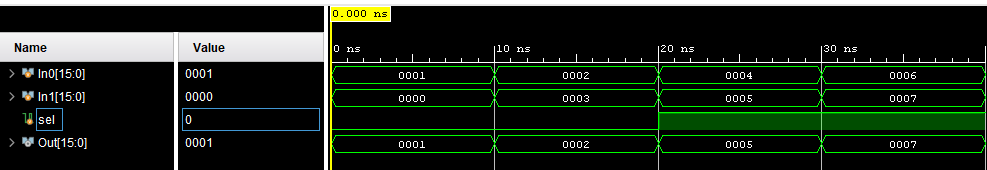
\includegraphics[width=1.0\textwidth]{Mux2_Test}
	\caption{Mux2 simulation waveform and ERT}
	\label{fig:sim_with_table}
\end{figure}

\begin{figure}[ht]\centering
	\begin{tabular}{l|rrrr}
		Time (ns): & 0 & 10 & 20 & 30  \\
		\midrule 
		In0 & 0 & 4 & 8 & c \\
		In1 & 1 & 5 & 9 & d  \\
		In2 & 2 & 6 & a & e  \\
		In3 & 3 & 7 & b & f  \\
		sel & 0 & 1 & z & 3  \\
		\bottomrule
		Out & 0 & 5 & a & f  \\
	\end{tabular}\medskip
	
	\includegraphics[width=1.0\textwidth]{Mux4_Test}
	\caption{Mux4 simulation waveform and ERT}
	\label{fig:sim_with_table}
\end{figure}

\begin{figure}[ht]\centering
	\begin{tabular}{l|rrrr}
		Time (ns): & 0 & 10 & 20 & 30 \\
		\midrule 
		In & 0 & 1 & 2 & 3  \\
		\bottomrule
		Out & e & d & b & 7 \\
	\end{tabular}\medskip
	
	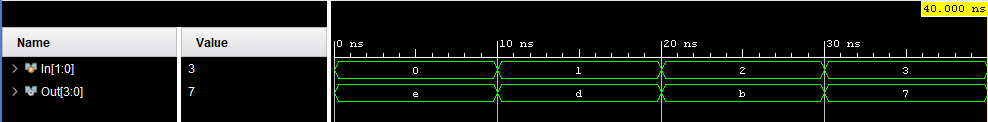
\includegraphics[width=1.0\textwidth]{annode_decoder_test}
	\caption{Annode decoder simulation waveform and ERT}
	\label{fig:sim_with_table}
\end{figure}

\begin{figure}[ht]\centering
	
	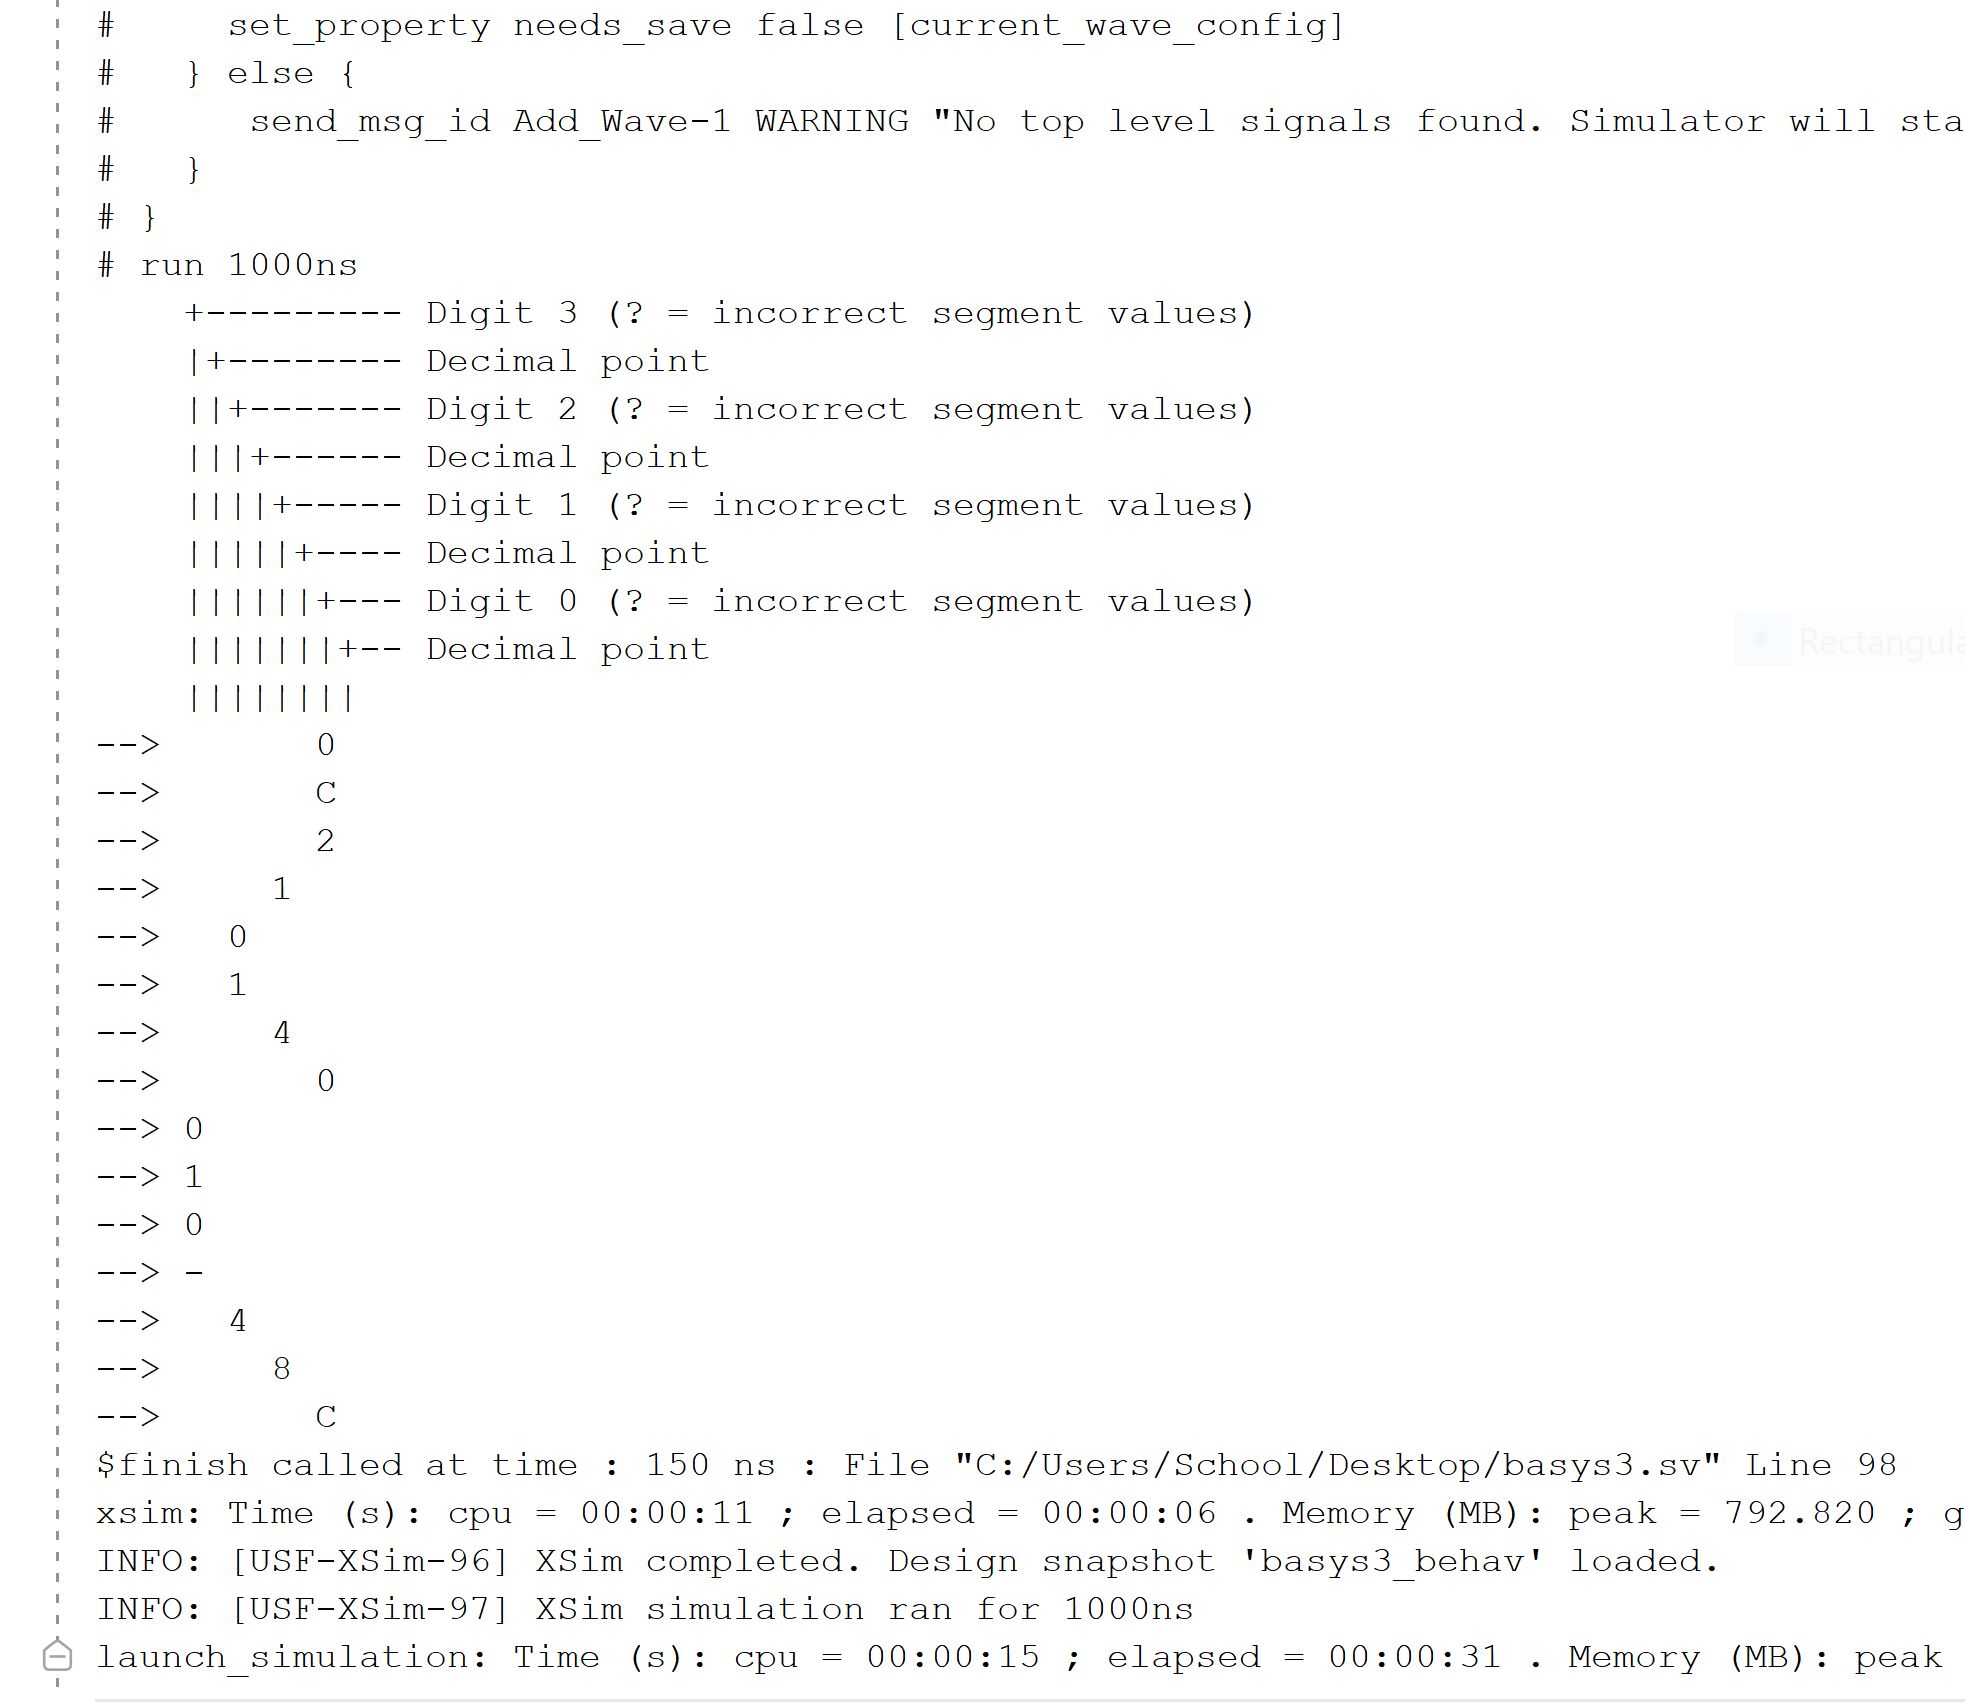
\includegraphics[width=1.0\textwidth]{TCL_Console}
	\caption{TCL Console output }
	\label{fig:sim_with_table}
\end{figure}


\clearpage


\section*{Code}

\begin{lstlisting}[style=Verilog,caption=Mux 2 Source File ,label=code:ex ]

// Jake Simmons and Chris Jones , ELC 2137, 2020 -3-24

module mux2 #(parameter N=2)(
input [N-1:0] in0, in1,
input sel,
output reg [15:0] out
);

always @*
case(sel)
0: out = in0 ;
default: out = in1 ;
endcase
endmodule



\end{lstlisting}

\begin{lstlisting}[style=Verilog,caption=Mux 2 Test Bench Code ,label=code:ex ]

// Jake Simmons and Chris Jones , ELC 2137, 2020 -3-24

module mux2_Test( );

reg [15:0] In0, In1;

reg sel;

wire [15:0] Out;

mux2 #(.N(16))  m1(

.in0(In0), .in1(In1),

.out(Out), .sel(sel)

);



initial begin

In0 = 16'b0000000000000000; In1 = 16'b0000000000000001; sel = 1'd0; #10;

In0 = 16'b0000000000000010; In1 = 16'b0000000000000011; sel = 1'd0; #10;

In0 = 16'b0000000000000100; In1 = 16'b0000000000000101; sel = 1'd1; #10;

In0 = 16'b0000000000000110; In1 = 16'b0000000000000111; sel = 1'd1; #10;



$finish;

end

endmodule




\end{lstlisting}



\begin{lstlisting}[style=Verilog,caption= Mux 4 Source File,label=code:ex ]

// Jake Simmons and Chris Jones , ELC 2137, 2020 -3-24

module mux4 #(parameter N =4)(
input [N-1:0] in0, in1, in2, in3,
input [1:0] sel,
output reg [3:0] out
);

always @*
case(sel)
0: out = in0;
1: out = in1;
2: out = in2;
default: out = in3;
endcase 
	  



\end{lstlisting}

\begin{lstlisting}[style=Verilog,caption= Mux 4 Test Bench Code,label=code:ex ]

// Jake Simmons and Chris Jones , ELC 2137, 2020 -3-24

module mux4_Test();
reg [3:0] in0, in1, in2, in3;
reg [1:0] sel; 
wire [3:0] out;

mux4 m4(
.in0(in0), .in1(in1), .in2(in2), .in3(in3), .sel(sel), .out(out)
);

initial begin
in0 = 4'b0000; in1 = 4'b0001; in2 = 4'b0010; in3 = 4'b0011; sel = 2'b00; #10;
in0 = 4'b0100; in1 = 4'b0101; in2 = 4'b0110; in3 = 4'b0111; sel = 2'b01; #10;
in0 = 4'b1000; in1 = 4'b1001; in2 = 4'b1010; in3 = 4'b1011; sel = 2'b10; #10;
in0 = 4'b1100; in1 = 4'b1101; in2 = 4'b1110; in3 = 4'b1111; sel = 2'b11; #10;

$finish;
end
endmodule



\end{lstlisting}

\begin{lstlisting}[style=Verilog,caption= Annode Decoder Source File,label=code:ex ]

// Jake Simmons and Chris Jones , ELC 2137, 2020 -3-24

module annode_decoder(
input [1:0] in,
output reg [3:0] out
);

always @*
case(in)
0: out = 4'b1110;
1: out = 4'b1101;
2: out = 4'b1011;
default: out = 4'b0111;
endcase
endmodule

\end{lstlisting}

\begin{lstlisting}[style=Verilog,caption= Annode Decoder Test Bench Code,label=code:ex ]

// Jake Simmons and Chris Jones , ELC 2137, 2020 -3-24

module annode_decoder_test();
reg [1:0] in;
wire [3:0] out;

annode_decoder ant(

.in(in), .out(out)
);

initial begin
in = 2'b00; #10;
in = 2'b01;  #10;
in = 2'b10;  #10;
in = 2'b11;  #10;

$finish;
end
endmodule

\end{lstlisting}


\begin{lstlisting}[style=Verilog,caption= Sseg4 Source File,label=code:ex ]
// Jake Simmons and Chris Jones , ELC 2137, 2020 -3-24

module sseg4(
input [15:0] data,
input hex_dec,
input sign,
input [1:0] digit_sel,
output [6:0] seg,
output dp,
output [3:0] an
);
wire [15:0] W1 ;
wire [15:0] W2 ;
wire [3:0] W3;
wire [6:0] W4;
wire [3:0] W5;
wire W6;
BCD11_2 B1( .in11(data[10:0]), .out11(W1));
mux2 #(.N(16)) B2( .in0(W1), .in1(data), .sel(hex_dec), .out(W2));
mux4 B3( .in0(W2[3:0]), .in1(W2[7:4]), .in2(W2[11:8]), .in3(W2[15:12]), .sel(digit_sel), .out(W3));
sseg_decoder B5( .num(W3), .sseg(W4));
mux2 #(.N(7)) B6( .in0(W4), .in1(7'b0111111), .out(seg) , .sel(W6));
and G2( W6, sign, ~W5[3]);
annode_decoder B7( .in(digit_sel), .out(W5));
assign dp = 1;
assign an = W5;
endmodule


\end{lstlisting}



\begin{lstlisting}[style=Verilog,caption=Sseg4 Manual Source File,label=code:ex ]
// Jake Simmons and Chris Jones , ELC 2137, 2020 -3-24

module sseg4_manual(
input [15:0] sw,
output [6:0] seg,
output dp,
output [3:0] an
);
sseg4 Sseg4(
.digit_sel(sw[13:12]), .sign(sw[14]), .hex_dec(sw[15]),
.data({4'b0000, sw[11:0]}), .seg(seg), .dp(dp), .an(an)
);
endmodule


\end{lstlisting}






\end{document}

